\documentclass{article}

\usepackage[cm]{fullpage}
\usepackage[russian]{babel}
\usepackage{amssymb}
\usepackage{amsmath}
\usepackage{setspace}
\usepackage{titlesec}
\usepackage{mdframed}
\usepackage{xcolor}
\usepackage{graphicx}
\usepackage{subcaption}
\usepackage{indentfirst}
\usepackage{titlesec}
\usepackage{accents}
\usepackage{hyperref}

\usepackage{float}

% Headers
\titleformat{\section}{\normalfont \Large \bfseries}{\thesection .}{0.2cm}{}
\titlespacing{\section}{0pt}{*-1}{*-1}

\titleformat{\subsection}{\normalfont \large \bfseries}{\thesubsection .}{0.2cm}{}
\titlespacing{\subsection}{3pt}{*-1}{*-2}

\titleformat{\subsubsection}{\normalfont \bfseries}{\thesubsubsection .}{0.2cm}{}
\titlespacing{\subsubsection}{6pt}{*-1}{*-2}

% Space between rows
\linespread{1.5}

% Space between paragraphs
\setlength{\parindent}{1cm}
\setlength{\parskip}{0.5cm}

% Commands
\newcommand{\R}{\mathbb R}
\newcommand{\E}[1]{\textsf E \left[ #1 \right]}
\newcommand{\Var}[1]{\textsf{Var} \left( #1 \right)}
\newcommand{\intR}{\int_{\R}}
\newcommand{\arc}[1]{\accentset{\smallsmile}{#1}}

% Operators


\begin{document}

\begin{center}
        {\bfseries \LARGE Individual Project}
\end{center}

\begin{center}
    \begin{flushleft}
        
            \vspace{-20pt}
            
            \textbf{Menadzhiev Maksim} \hfill \textbf{FES, 2023-2024}
            
            \vspace{-30pt}
            
            \hrulefill
 
    \end{flushleft}
\end{center}


% Part 1
\section{INTRODUCTION}

% Part 2
\section{STOCHASTIC MODEL FOR MEDIA ATTENTION}

\subsection{MEDIA ATTENTION INDEX}
To begin with, lets introduce the media attention index

\[M_{t} = \exp \left\{ {\mu t + \sigma W_{t} + \sum \limits_{i=1}^{N_{t}} \xi{i}} \right\}, \quad t \geq 0,\] where $W_{t}$ - a Wiener process, $\sum \limits_{i=1}^{N_{t}} \xi_{i}$ - a compound Poisson process such that $N_{t}$ is a homogeneous Poisson process with intensity $\lambda$ and $\xi_{1}, \xi_{2},$... are i.i.d. r.v. with absolutely continuous distribution having the density $p$.

\subsection{WHY EXPONENT?}

First of all, I would like to notice that, as I understand, the main reason for using exponent is the exclusion of negative values of $M_{t}$ that don't make sense while $W_{t}$ and $\sum \limits_{i=1}^{N_{t}} \xi_{i}$ can be negative.

\subsection{WHAT IS THE SENSE OF $\boldsymbol{D_{k}}$?}
 
 We have the discrete grid $0, \Delta, 2\Delta, ...  $ with fixed $\Delta > 0$ on which $M_{t}$ is considered.
 Now lets introduce
 \[D_{k} := \log M_{k \Delta} - \log M_{(k - 1) \Delta}, \quad k = 1, 2, ... \]
 with $\log M_{0} = 0$ what means that $M_{0} = 1$. Thus due to properties of the logarithm $D_{k}$ can be submitted as \[D_{k} = \log \frac{M_{k \Delta}} {M_{(k - 1) \Delta}}, \quad k = 1, 2, ...,\] where $\frac {M_{k \Delta}} {M_{(k - 1) \Delta}}$ is the growth of $M_{t}$ during period $k$. So in this case we are considering the change of $M_{t}$ and it would be great, if we could somehow model it.
 
\subsection{WHAT PROCESS IS $\boldsymbol{\log{M_{k \Delta}}}$?}
 
The first obvious observation is that \[\log M_{k \Delta} = \mu k \Delta + \sigma W_{k \Delta} + \sum \limits_{i=1}^{N_{k \Delta}} \xi_{i} \Rightarrow D_{k} = \mu \Delta + \sigma (W_{k \Delta} - W_{(k - 1) \Delta})  + \sum \limits_{i=1}^{N_{k \Delta}} \xi_{i} - \sum \limits_{i=1}^{N_{(k - 1) \Delta}} \xi_{i},\] where $W_{k \Delta} - W_{(k - 1) \Delta} \sim N(0, \Delta)$ and the characteristic function of $\sum \limits_{i=1}^{N_{k \Delta}} \xi_{i} - \sum \limits_{i=1}^{N_{(k - 1) \Delta}} \xi_{i}$ is $\exp\{  \lambda \Delta (\phi_{\xi}(u) - 1) \}$.
 
Also it makes sense to understand what process $\log{M_{k \Delta}}$ is. The most promising suggestion is that $\log M_{k \Delta}$ is a L\'evy process. So then $D_{k}$ is an increment of a L\'evy process, therefore, $\forall i, j = 0, 1, 2, ... : i \neq j: \;  D_{i \Delta} \text{ and } D_{j \Delta}$ are independent.

As we saw before $\log M_{k \Delta} = \mu k \Delta + \sigma W_{k \Delta} + \sum \limits_{i=1}^{N_{k \Delta}} \xi_{i}$ - a sum of a Brownian motion, a compound Poisson process which are known to be L\'evy processes and a non-stochastic part. Thus, taking into an account that $\log M_{0} = 0$ we also get that $\log M_{k \Delta}$ has independent increments and it is stochastic continious.

Therefore, $\log M_{k \Delta}$ is a L\'evy process and $D_{k}$ represents its increments.

$\mathbf{NB:}$\begin{enumerate}
    \item \text{Since we can get $D_k$ from the real data, thus it is a sample} \\
    \item \text{A jump in $\log M_{\Delta}$ is caused only by an increment in the CPP beacause other parts are continious}
\end{enumerate}

\subsection{THE L\'EVY-KHINCHINE FORMULA}

Let us write the L\'evy-Khinchine formula in general terms. Let $X_{t}$ be a L\'evy process. Then \[ \phi_{t}(u) = \mathbb{E}[e^{iu X_{t}}] = \exp \{t (i u b - \frac{1} {2} c^2 u^2 + \int_{\mathbb{R}} (e^{iux} - 1 - i u x \mathbb{I} \{|x| < 1\}) \nu(dx)) \}, \] where  $b \in \mathbb{R}, \, c \in \mathbb{R}_{+}$ and $\nu$ is a L\'evy measure of $X_{t}$.

So if we take into account that $\nu(dx) = \lambda p_{\xi}(x)$, consideration the integral in this formula gives us \[ \int_{\mathbb{R}} (e^{iux} - 1 - i u x \mathbb{I} \{|x| < 1\}) \nu(dx) = \int_{\mathbb{R}} (e^{iux} - 1) \nu(dx) - i u  \int_{\mathbb{R}} x \mathbb{I} \{|x| < 1\} \nu(dx) \] because \[ \text{1) } \int_{\mathbb{R}} (e^{iux} - 1) \nu(dx) = \int_{|x| < 1} (e^{iux} - 1) \nu(dx) + \int_{|x| \geq 1} (e^{iux} - 1) \nu(dx) \leq \] \[ \leq ||\; e^{i u x} - 1 \leq |e^{i u x} - 1| \leq |e^{i u x}| + 1 = 2 \text{ and } \int_{|x| < 1} (e^{iux} - 1) \nu(dx) \text{ is finite} \; || \leq 2 \int_{|x| \geq 1} \nu(dx) \] \[ \text{2) } \int_{\mathbb{R}} x \mathbb{I} \{|x| < 1\} \nu(dx) = \int_{|x| < 1} x  \nu(dx) \leq \int_{|x| < 1} |x| \nu(dx) \leq  \int_{|x| < 1} \nu(dx) \]
thus, both parts of the integral are finite. Therefore \[ \phi_{t}(u) =  \exp \{t (i u b - \frac{1} {2} c^2 u^2 + \int_{\mathbb{R}} (e^{iux} - 1) \nu(dx) - i u  \int_{\mathbb{R}} x \mathbb{I} \{|x| < 1\}) \nu(dx)) \} = \] \[= \exp \{t (i u (b - \int_{\mathbb{R}} x \mathbb{I} \{|x| < 1\} \nu(dx)) - \frac{1} {2} c^2 u^2 + \int_{\mathbb{R}} (e^{iux} - 1) \nu(dx)) \} \]

So if \[ \mu = b - \int_{\mathbb{R}} x \mathbb{I} \{|x| < 1\} \nu(dx) \text { and } \sigma = c, \] then in our case the characteristic function of $\log M_{\Delta}$ is \[ \phi_{\Delta}(u) = \mathbb{E}[e^{i u \log M_{\Delta}}] = \exp \{\Delta \bigr(i \mu u - \frac{1} {2} \sigma^2 u^2 + \int_{\mathbb{R}}(e^{iux} - 1) \nu(dx) \bigr) \} = \exp \{\Delta \bigr(i \mu u - \frac{1} {2} \sigma^2 u^2 + \lambda \int_{\mathbb{R}}e^{iux} p_{\xi}(x) dx - \lambda \int_{\mathbb{R}} p_{\xi}(x) dx \bigr) \} = \] \[ = \exp \{ \Delta \bigr(i \mu u - \frac{1} {2} \sigma^2 u^2 - \lambda + \lambda \mathcal{F}[p](u) \bigr) \}, \; u \in \mathbb{R}, \] where $\nu(dx) = \lambda p_{\xi}(x) dx$ and $\mathcal{F}[p](u) = \int_{\mathbb{R}}e^{iux} p_{\xi}(x) dx$

% Part 3
\section{ESTIMATION OF MEDIA ATTENTION}

\subsection{APPROACH TO ESTIMATION}

In what follows, we use function \[ \varphi_{\Delta}(u) := \frac{1}{\Delta} \log(\phi_{\Delta}(u)) = i u \mu - \frac{1}{2} \sigma^2 u^2 - \lambda + \lambda \mathcal{F}[p](u), \quad u \in \mathbb{R}. \]

Due to the Riemann-Lebesque lemma, $\mathcal{F}[p](u) \rightarrow 0$ as $|u| \rightarrow \infty$. Therefore, \[ \begin{aligned}
    & Re(\varphi_{\Delta}(u)) = -\frac{1}{2} \sigma^2 u^2 - \lambda + o(1) \\
    & Im(\varphi_{\Delta}(u)) = u \mu + o(1),
\end{aligned} \] as $|u| \rightarrow \infty$. So in estimation we should use only large $u$.

\definecolor{paleblue}{RGB}{0, 0, 255}
\colorlet{paleblue}{blue!20!white}

\begin{mdframed}[linecolor=black, backgroundcolor=paleblue]
    \textbf{Complex logarithm}
    
    One should consider $z = x + i y = r e^{i \varphi}$, where $r = \sqrt{x^2 + y^2}$ is an absolute value of $z$, and $\varphi$ is its argument.
    
    Obviously $\tan{\varphi} = \frac{y}{x} \Rightarrow \varphi = \arctan{\frac{y}{x}}$.
    
    Then $\log{z} = \log r + i \varphi = \log{\sqrt{x^2 + y^2}} + i \arctan{\frac{y}{x}}$
\end{mdframed}

It is known that mathematical expectation can be estimated by mean value then a natural estimation of $\varphi_{\Delta}(u)$ is \textbf{(don't know why $D_k$)}
\[
\hat{\varphi}_{\Delta}(u) := \frac{1}{\Delta} \log(\frac{1}{n} \sum\limits_{k=1}^n e^{i u D_k}) = -\frac{1}{\Delta} \log n + \frac{1}{\Delta} \log{\sum\limits_{k=1}^n e^{i u D_k}} = -\frac{1}{\Delta} \log n + \frac{1}{\Delta} \log{(\sum\limits_{k=1}^n \cos(u D_k) + i \sum\limits_{k=1}^n \sin(u D_k))} =
\]
\[ = -\frac{1}{\Delta} \log n + \frac{1}{\Delta} \left( \frac{1}{2} \log \left[\left(\sum\limits_{k=1}^n \cos(u D_k)\right)^2 + \left(\sum\limits_{k=1}^n \sin(u D_k)\right)^2  \right] + i \arctan \left( \frac{\sum_{k=1}^n \sin(u D_k)} {\sum_{k=1}^n \cos(u D_k)} \right) \right) = 
\]
\[ =  -\frac{1}{\Delta} \log n + \frac{1} {2 \Delta} \log \left[\left(\sum\limits_{k=1}^n \cos(u D_k)\right)^2 + \left(\sum\limits_{k=1}^n \sin(u D_k)\right)^2  \right] + i \frac{1}{\Delta} \arctan \left( \frac{\sum_{k=1}^n \sin(u D_k)} {\sum_{k=1}^n \cos(u D_k)} \right), \quad u \in \mathbb{R}.
\]

Thus, for large $u$ it makes sense to consider \textbf{(don't know the sense of $w^{U_n}(u)$)}
\begin{enumerate}
    \item $\int_{\mathbb{R}_+} w^{U_n}(u) \left[ Re(\hat{\varphi}_{\Delta}(u)) - (-\frac{1}{2} \sigma^2 u^2 - \lambda) \right]^2 du = \int_{\mathbb{R}_+} w^{U_n}(u) \left[ Re(\hat{\varphi}_{\Delta}(u)) + \frac{1}{2} \sigma^2 u^2 + \lambda \right]^2 du$
    
    \item $\int_{\mathbb{R}_+} w^{V_n}(u) \left[ Im(\hat{\varphi}_{\Delta}(u)) - \mu u \right]^2 du$
\end{enumerate}

Therefore,
\begin{enumerate}
    \item $(\hat{\sigma}^2, \; \hat{\lambda}^2) = \underset{\sigma^2, \, \lambda}{arg \min} \int_{\mathbb{R}_+} w^{U_n}(u) \left[ Re(\hat{\varphi}_{\Delta}(u)) + \frac{1}{2} \sigma^2 u^2 + \lambda \right]^2 du \overset{?}{=} \underset{\sigma^2, \, \lambda}{arg \min} \int_{\varepsilon}^1 w(u)  \left[ Re(\hat{\varphi}_{\Delta}(u U_n)) + \frac{1}{2} \sigma^2 u^2 U_n^2 + \lambda \right]^2 du $
    
    \item $\hat{\mu} = \underset{\mu}{arg \min} \int_{\mathbb{R}_+} w^{V_n}(u) \left[ Im(\hat{\varphi}_{\Delta}(u)) - \mu u \right]^2 du \overset{?}{=}  \underset{\mu}{arg \min} \int_{\varepsilon}^1 w(u) \left[ Im(\hat{\varphi}_{\Delta}(u V_n)) - \mu u V_n \right]^2 du$
\end{enumerate}

\subsection{ALGORITHM 1}

\[ Q_1(\sigma^2, \lambda) = \sum\limits_{j=1}^{N} w(\tilde{u}_j) \left[ Re(\hat{\varphi}_{\Delta}(\tilde{u}_j U_n)) + \frac{1}{2} \sigma^2 \tilde{u}_j^2 U_n^2 + \lambda \right]^2 \longrightarrow \underset{\sigma^2, \lambda}{\min} \]

So one needs to consider \[ \begin{cases}
    \frac{\partial Q_1(\sigma^2, \, \lambda)}{\partial \sigma^2} = \sum\limits_{j=1}^{N} w(\tilde{u}_j) \tilde{u}_j^2 U_n^2 \left[ Re(\hat{\varphi}_{\Delta}(\tilde{u}_j U_n)) + \frac{1}{2} \sigma^2 \tilde{u}_j^2 U_n^2 + \lambda \right] = 0 \\
    \frac{\partial Q_1(\sigma^2, \, \lambda)}{\partial \lambda} = \sum\limits_{j=1}^{N} w(\tilde{u}_j) \left[ Re(\hat{\varphi}_{\Delta}(\tilde{u}_j U_n)) + \frac{1}{2} \sigma^2 \tilde{u}_j^2 U_n^2 + \lambda \right] = 0
\end{cases} \Leftrightarrow \]
\[ \Leftrightarrow \begin{cases}
    \sum\limits_{j=1}^{N} w(\tilde{u}_j) Re(\hat{\varphi}_{\Delta}(\tilde{u}_j U_n)) (\tilde{u}_j U_n)^2 + \frac{\sigma^2}{2} U_n^4 \sum\limits_{j=1}^{N} w(\tilde{u}_j)\tilde{u}_j^{2 \cdot 2} + \lambda U_n^2 \sum\limits_{j=1}^{N} w(\tilde{u}_j) \tilde{u}_j^2 = 0 \\
     \sum\limits_{j=1}^{N} w(\tilde{u}_j) Re(\hat{\varphi}_{\Delta}(\tilde{u}_j U_n)) + \frac{\sigma^2}{2} U_n^2 \sum\limits_{j=1}^{N} w(\tilde{u}_j)\tilde{u}_j^{2} + \lambda \sum\limits_{j=1}^{N} w(u_j) = 0_.
\end{cases} \]

Let \[ \begin{aligned}
    & \Lambda_d = \sum\limits_{j=1}^{N} w(\tilde{u}_j) \tilde{u}_j^{2d}, \; d = 0, 1, 2 \\
    & \Psi_d = \sum\limits_{j=1}^N w(\tilde{u}_j) Re(\hat{\varphi}_{\Delta}(\tilde{u}_j U_n))(\tilde{u}_j U_n)^{2d}, \; d = 0, 1
\end{aligned} \]

Therefore, \[ \begin{cases}
    \Psi_1 + \frac{\sigma^2}{2} U_n^4 \Lambda_2 + \lambda U_n^2 \Lambda_1 = 0 \\
    \Psi_0 + \frac{\sigma^2}{2} U_n^2 \Lambda_1 + \lambda \Lambda_0 = 0
\end{cases} \Leftrightarrow \begin{cases}
    \sigma^2_n = 2 \frac{\Psi_0 \Lambda_1 U_n^2 - \Psi_1 \Lambda_0}{(\Lambda_2 \Lambda_0 - \Lambda_1^2) U_n^4} \\
    \lambda_n = \frac{\Psi_1 \Lambda_1 - \Psi_0 \Lambda_2 U_n^2}{(\Lambda_2 \Lambda_0 - \Lambda_1^2) U_n^2}
\end{cases} \]

\subsection{ALGORITHM 2}

Considering the function \[ \varphi_{\Delta}(u) := \frac{1}{\Delta} \log(\phi_{\Delta}(u)) = i u \mu - \frac{1}{2} \sigma^2 u^2 - \lambda + \lambda \mathcal{F}[p](u), \quad u \in \mathbb{R} \] provides for us a representation of the density $p$ as follows \[ \lambda \mathcal{F}[p](u) = \varphi_{\Delta}(u) - i u \mu + \frac{1}{2} \sigma^2 u^2 + \lambda \Rightarrow \hat{p}_n (x) = \hat{\mathcal{F}}^{-1} \left( \frac{1}{\hat{\lambda}} (\hat{\varphi}_{\Delta}(u) - i u \hat{\mu} + \frac{1}{2} \hat{\sigma}^2 u^2 + \hat{\lambda}) K(u / T_n) \right) = \]
\[ = \frac{1}{2 \pi \hat{\lambda}} \int_{\mathbb{R}} e^{-i u x} \left( \hat{\varphi}_{\Delta}(u) - i u \hat{\mu} + \frac{1}{2} \hat{\sigma}^2 u^2 + \hat{\lambda} \right) K(u / T_n) du \] as an inverse Fourier transform, where $K: \mathbb{R} \rightarrow \mathbb{R}_+$ is a smoothing kernel \[ K(x) = \begin{cases}
    1, & |x| < 0.05 \\
    exp \left\{ -\frac{e^{-1 / (|x| - 0.05)}} {1 - |x|} \right\} , & 0.05 < |x| < 1 \\
    0, & |x| > 1_.
\end{cases} \]

Then according to \textit{algorithm 2} one should take points $u_j \in [-1, 1], \; j = 1, ..., N.$ Therefore if $u$ in the theoretical case is an analog of $u_j$ \[ \hat{p}_n (x) = \frac{1}{2 \pi \hat{\lambda}} \int\limits_{-1}^{1} e^{-i (u T_n) x} \left( \hat{\varphi}_{\Delta}(u T_n) - i (u T_n) \hat{\mu} + \frac{1}{2} \hat{\sigma}^2 (u T_n)^2 + \hat{\lambda} \right) K(u) d(u T_n) \] can be represented in discrete form as \[ \hat{p}_n (x_s) = \frac{T_n \delta}{2 \pi \hat{\lambda}} \sum\limits_{j=1}^{N} e^{-i \arc{u}_j x_s} \left( \hat{\varphi}_{\Delta}(\arc{u}_j) - i \arc{u}_j \hat{\mu} + \frac{1}{2} \hat{\sigma}^2 \arc{u}_{j}^2 + \hat{\lambda} \right) K(\arc{u}_j / T_n). \]


\subsection{SIMULATION  STUDY}

Let us consider the Merton jump-diffusion model \[ M_t = \exp \left\{\mu t + \sigma W_t + \sum\limits_{i=1}^{N_t} \xi_i \right\}, \] where $W_t \sim N(0, t), N_t \sim Pois(\lambda t)$ and $\xi_i \sim N(0, 1)$.

For further calculations I have taken 25 samples and the parameters have been chosen to be $\mu = 0, \sigma = 1, \lambda = 10$ and $\Delta = 0.1$. Therefore, if $n$ is the size of a sample we will use $\{0, \, 0.1, \, 0.2, ..., 0.1 \, n\}$ grid.


\subsubsection{BROWNIAN MOTION}

Note that $B_{k \Delta} = \sum\limits_{j=1}^k \left[ B_{j \Delta} - B_{(j - 1) \Delta} \right]$, where $B_{j \Delta} - B_{(j - 1)} \sim N(0, \; \Delta).$ So we can calculate the value of $B_{k\Delta}$ in each point.

\begin{figure}[H]
    \centering
    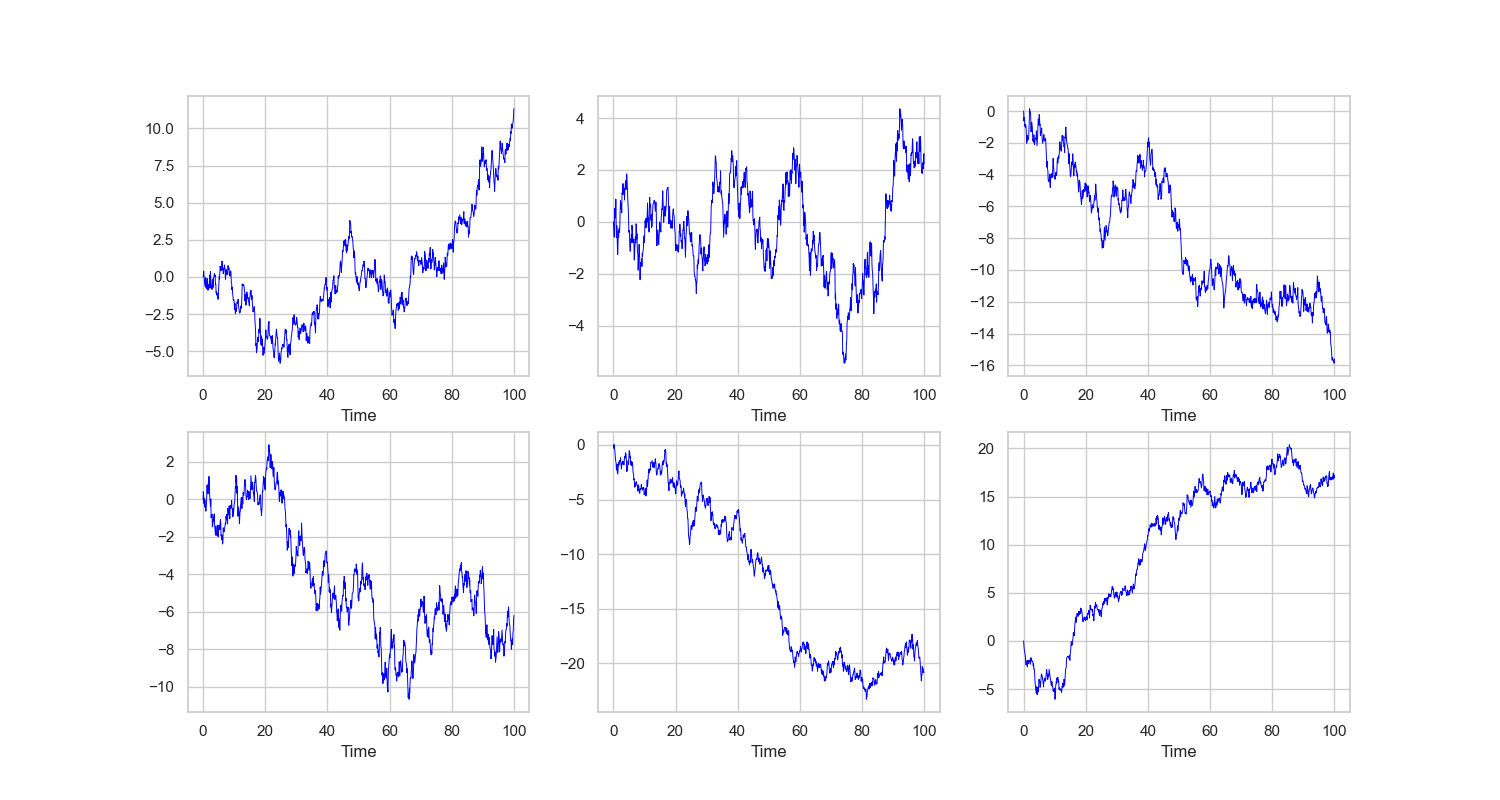
\includegraphics[width=\textwidth]{/Users/mmenadzhiev/Desktop/Studying/Project/Estimation of the media attention/Data/Brownian motion.png}
    \caption{Trajectory of $B_{k\Delta}$}
\end{figure}

\subsubsection{POISSON PROCESS}

Similarly $N_{k \Delta} = \sum\limits_{j=1}^{k} \left[ N_{j \Delta} - N_{(j - 1) \Delta} \right]$, where $N_{j \Delta} - N_{(j - 1) \Delta} \sim Pois(\lambda \Delta)$.
\begin{figure}[H]
    \centering
    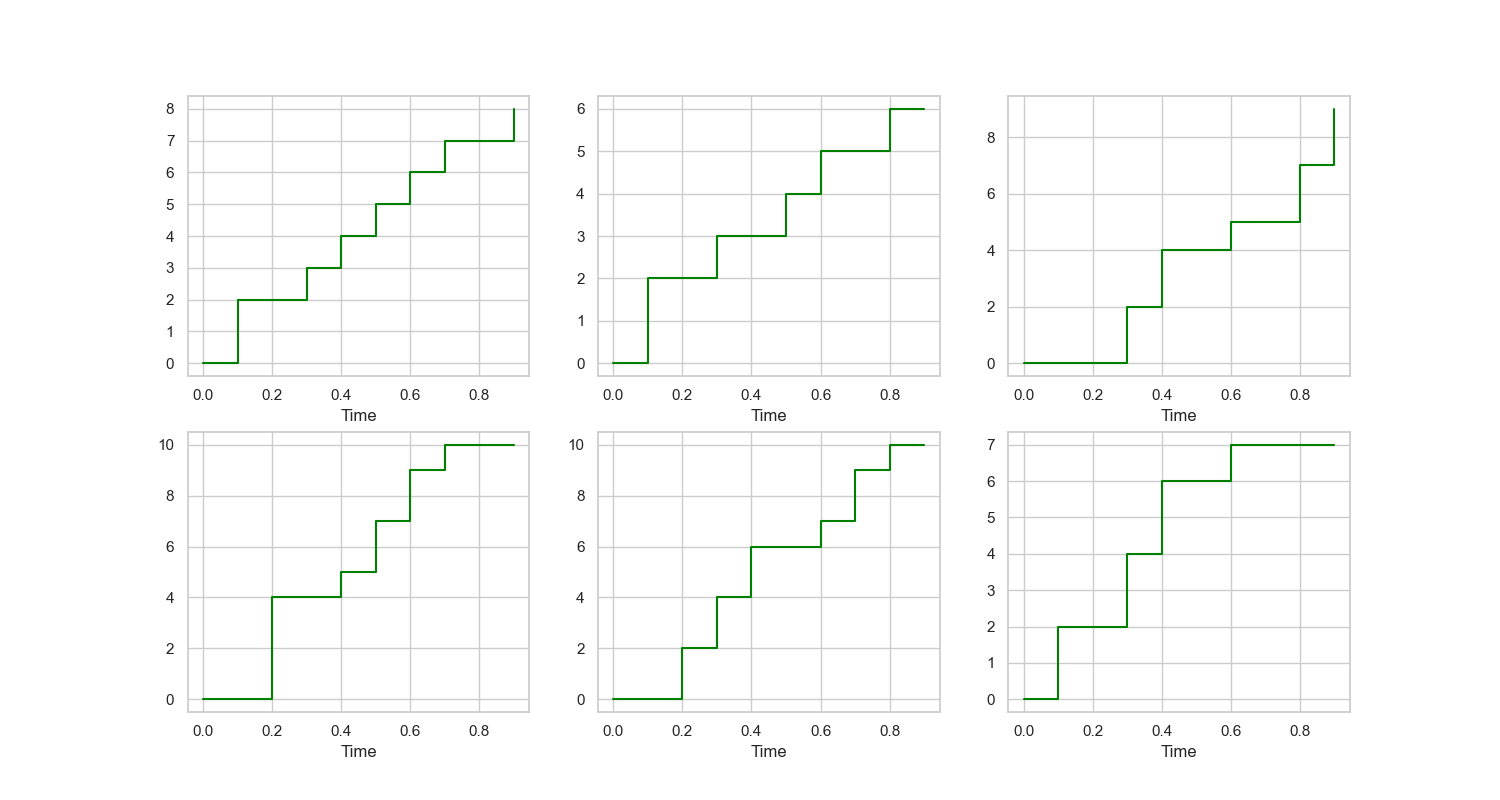
\includegraphics[width=\textwidth]{/Users/mmenadzhiev/Desktop/Studying/Project/Estimation of the media attention/Data/Poisson process.png}
    \caption{Trajectories of $N_{k\Delta}$}
\end{figure}

\subsubsection{COMPOUND POISSON PROCESS}

Now we have everything for counting values of Compound Poisson process $\sum\limits_{i=1}^{N_{k\Delta}} \xi_i$.

\begin{figure}[H]
    \centering
    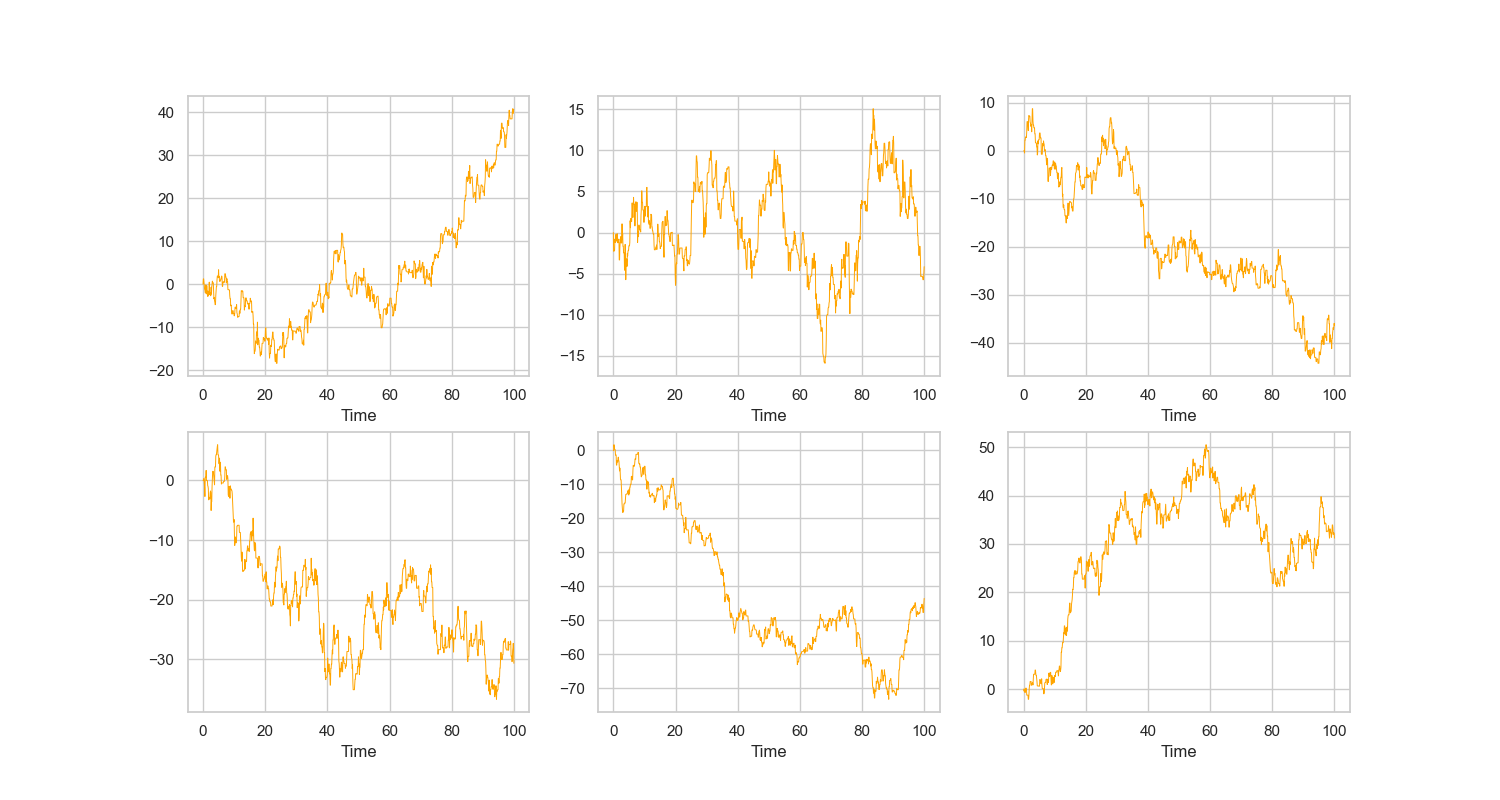
\includegraphics[width=\textwidth]{/Users/mmenadzhiev/Desktop/Studying/Project/Estimation of the media attention/Data/CPP.png}
    \caption{Trajectories of $\sum\limits_{i=1}^{N_{k\Delta}} \xi_i$}
\end{figure}

\subsubsection{$\boldsymbol{M_{k \Delta}}$ and $\boldsymbol{\log M_{k \Delta}}$}

\begin{figure}[htbp]
    \centering
    \begin{subfigure}{0.45\textwidth}
        \centering
        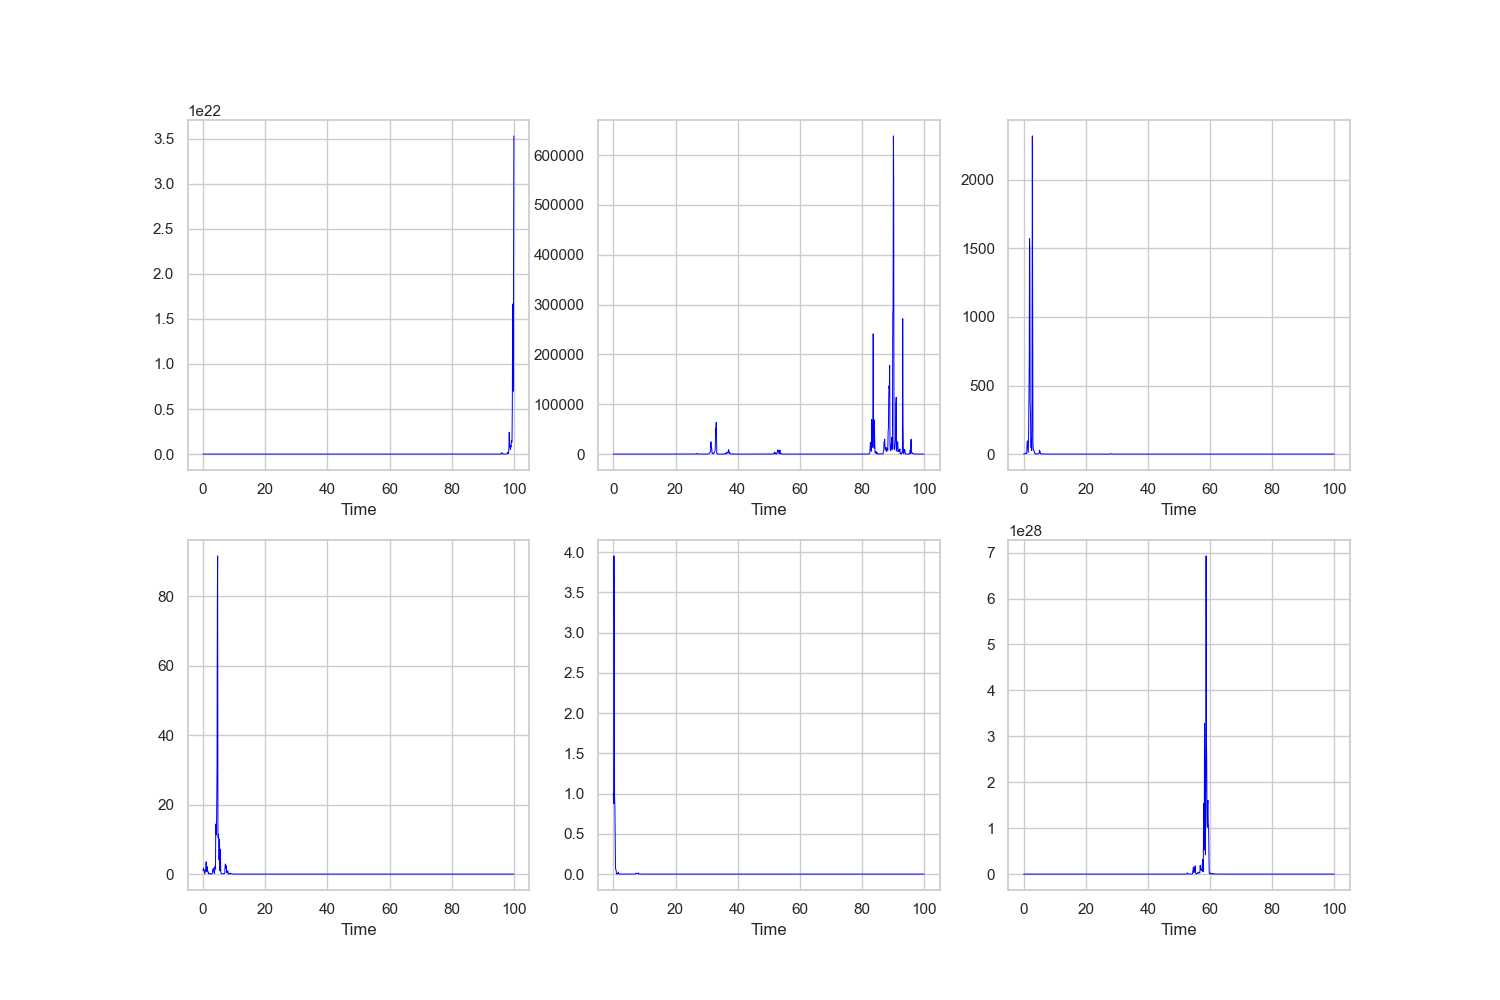
\includegraphics[width=\linewidth]{/Users/mmenadzhiev/Desktop/Studying/Project/Estimation of the media attention/Data/M_kDelta.png}
        \caption{ $M_{k \Delta}$}
        \label{fig:sub1}
    \end{subfigure}
    \begin{subfigure}{0.45\textwidth}
        \centering
        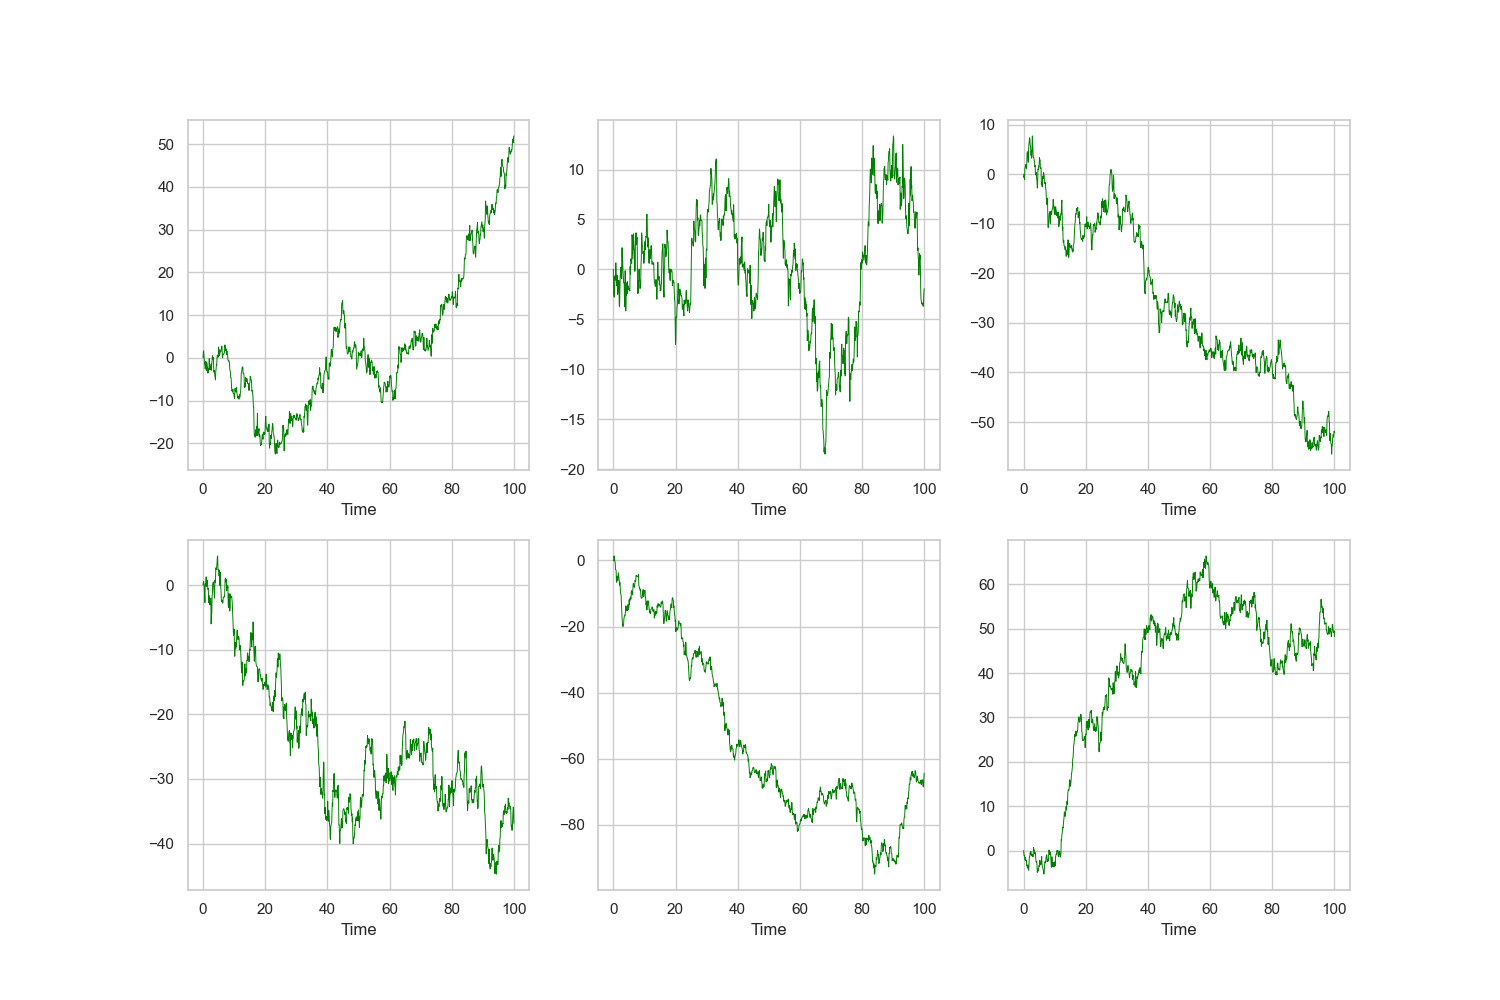
\includegraphics[width=\linewidth]{/Users/mmenadzhiev/Desktop/Studying/Project/Estimation of the media attention/Data/logM_kDelta.png}
        \caption{$\log {M_{k \Delta}}$}
        \label{fig:sub2}
    \end{subfigure}
    \caption{Graphs of $M_{k \Delta}$ and $\log {M_{k \Delta}}$}
    \label{fig:main}
\end{figure}


\subsubsection{CALCULATIONS}

As it has been said before, we consider \[ M_t = \exp \left\{\mu t + \sigma W_t + \sum\limits_{i=1}^{N_t} \xi_i \right\} \] and for each point of grid $\{ k \Delta\}_{k=0}^{n}  =  \{0, \, 0.1, \, 0.2, ..., \, 0.1 \, n \}$ the values of $W_{k \Delta}$ and $\sum\limits_{i=1}^{N_{k\Delta}} \xi_i$ then $M_{k \Delta}$ can be counted. To be more precise, \[ M_{k \Delta} = \exp \left\{\mu k \Delta + \sigma W_{k \Delta} + \sum\limits_{i=1}^{N_{k \Delta}} \xi_i \right\} \]

Thus, we can also get $D_k = \log M_{k \Delta} - \log M_{(k - 1) \Delta_.}$

\textbf{Approximate $Re(\varphi_{\Delta}(u))$}

As $|u| \rightarrow \infty$ approximately
$$
\varphi_{\Delta}(u) \approx i \mu u - \frac{1}{2} \sigma^2 u^2 - \lambda \Rightarrow Re(\varphi_{\Delta}(u)) \approx - \frac{1}{2} \sigma^2 u^2 - \lambda \text{ (denoted as \textit{re\_approx})}
$$

\textbf{Estimated $Re(\varphi_{\Delta}(u))$}

We found before that \[ \hat{\varphi}_{\Delta}(u) = -\frac{1}{\Delta} \log n + \frac{1}{2 \Delta} \log \left[ \left( \sum\limits_{k=1}^n \cos(u D_k) \right)^2 + \left(\sum\limits_{k=1}^n \sin(u D_k) \right)^2 \right] + i \frac{1}{\Delta} \arctan \left(\frac{\sum_{k=1}^n \sin(u D_k))}{\sum_{k=1}^n \cos(u D_k)} \right) \Rightarrow \] \[ \Rightarrow Re(\hat{\varphi}_{\Delta}(u)) = -\frac{1}{\Delta} \log n + \frac{1}{2 \Delta} \log \left[ \left( \sum\limits_{k=1}^n \cos(u D_k) \right)^2 + \left(\sum\limits_{k=1}^n \sin(u D_k) \right)^2 \right] \text{ (denoted as \textit{re\_hat)}} \]

\textbf{Factual $Re(\varphi_{\Delta}(u))$}

To find factual real part of $\varphi_{\Delta}(u) = \frac 1 \Delta \log \phi_{\Delta}(u)$ one should remember that in our case $\xi_i \sim \mathcal{N}(0, 1)$. Thus, $p_{\xi}(x) = \frac {1} {\sqrt{2 \pi}} e^{- \frac {x^2} {2}}$. Then \[ \varphi_{\Delta}(u) = i \mu u - \frac 12 \sigma^2 u^2 + \int_{\R} (e^{iux} - 1) \nu(x) =  i \mu u - \frac 12 \sigma^2 u^2 + \lambda \int_{\R} e^{iux} p_{\xi}(x) dx - \lambda \int_{\R} p_{\xi}(x) dx =  i \mu u - \frac 12 \sigma^2 u^2 - \lambda + \frac{\lambda}{\sqrt{2 \pi}} \int_{\R} e^{-\frac{x^2}{2} + iux} dx = \] \[ = i \mu u - \frac 12 \sigma^2 u^2 - \lambda + \lambda e^{-\frac{u^2}{2}}. \]

Therefore \[ Re(\varphi_{\Delta}(u)) = - \frac 12 \sigma^2 u^2 - \lambda + \lambda e^{-\frac{u^2}{2}} \text{ (denoted as \textit{re\_fact}).} \]

So for $n = 1000$ we can observe
\begin{figure}[H]
    \centering
    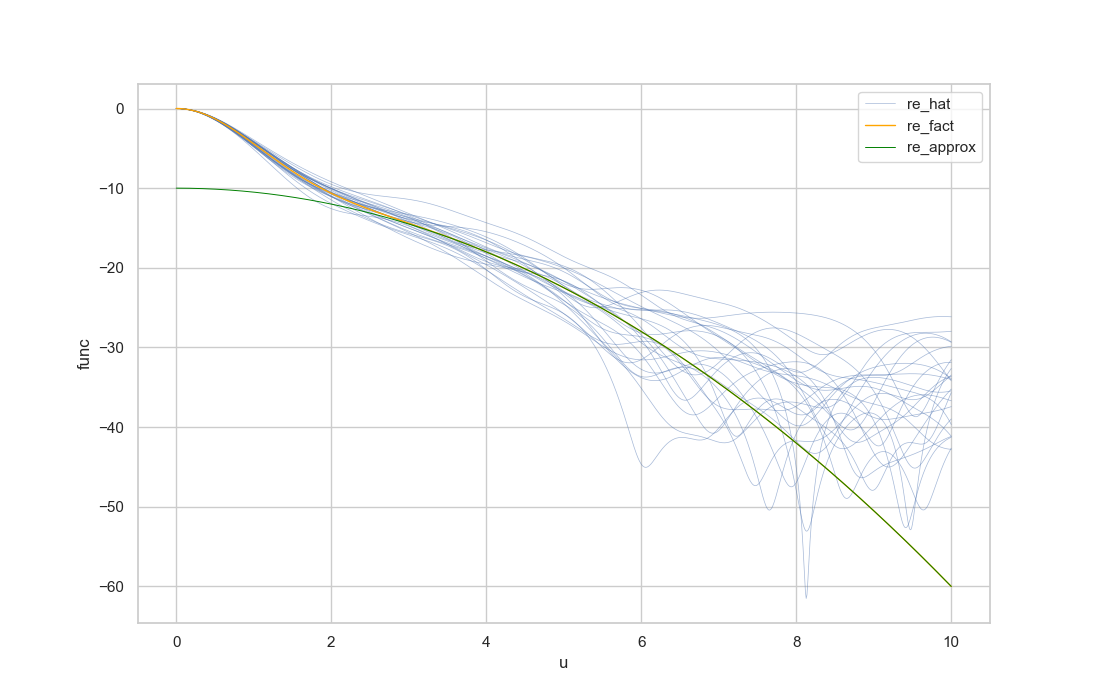
\includegraphics[width=\textwidth]{/Users/mmenadzhiev/Desktop/Studying/Project/Estimation of the media attention/Data/Real parts.png}
    \caption{Factual, approximate and estimated real parts of $\varphi_{\Delta}(u)$}
\end{figure}

And it can be seen that all three lines are close to each other when $u \in [3, 6]$. Therefore, it makes sense to take $\varepsilon = 0.5, U_n  = V_n = 6$.


After all calculations I received
\begin{figure}[H]
    \centering
    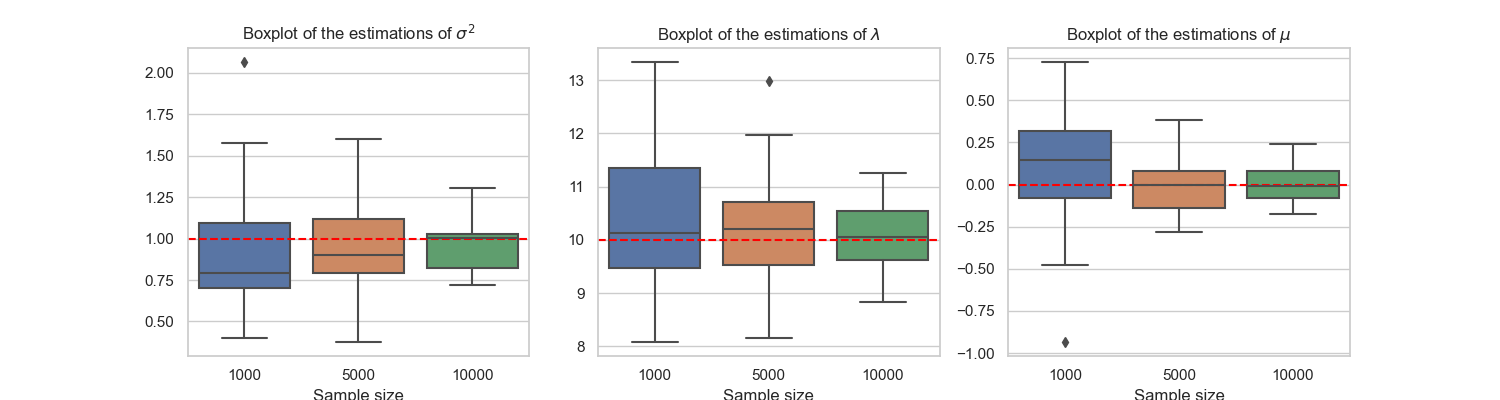
\includegraphics[width=\textwidth]{/Users/mmenadzhiev/Desktop/Studying/Project/Estimation of the media attention/Data/boxplots.png}
    \caption{Boxplots of the estimations of $\sigma^2, \lambda$ and $\mu$}
\end{figure}

As for the density's estimation I have taken $T_n = 3.3$ and $m = 100$ points between $-5$ and $5$ as $x_s$. The result which I  have got according to algorithm 2 is presented in figure 7.

\begin{figure}[H]
    \centering
    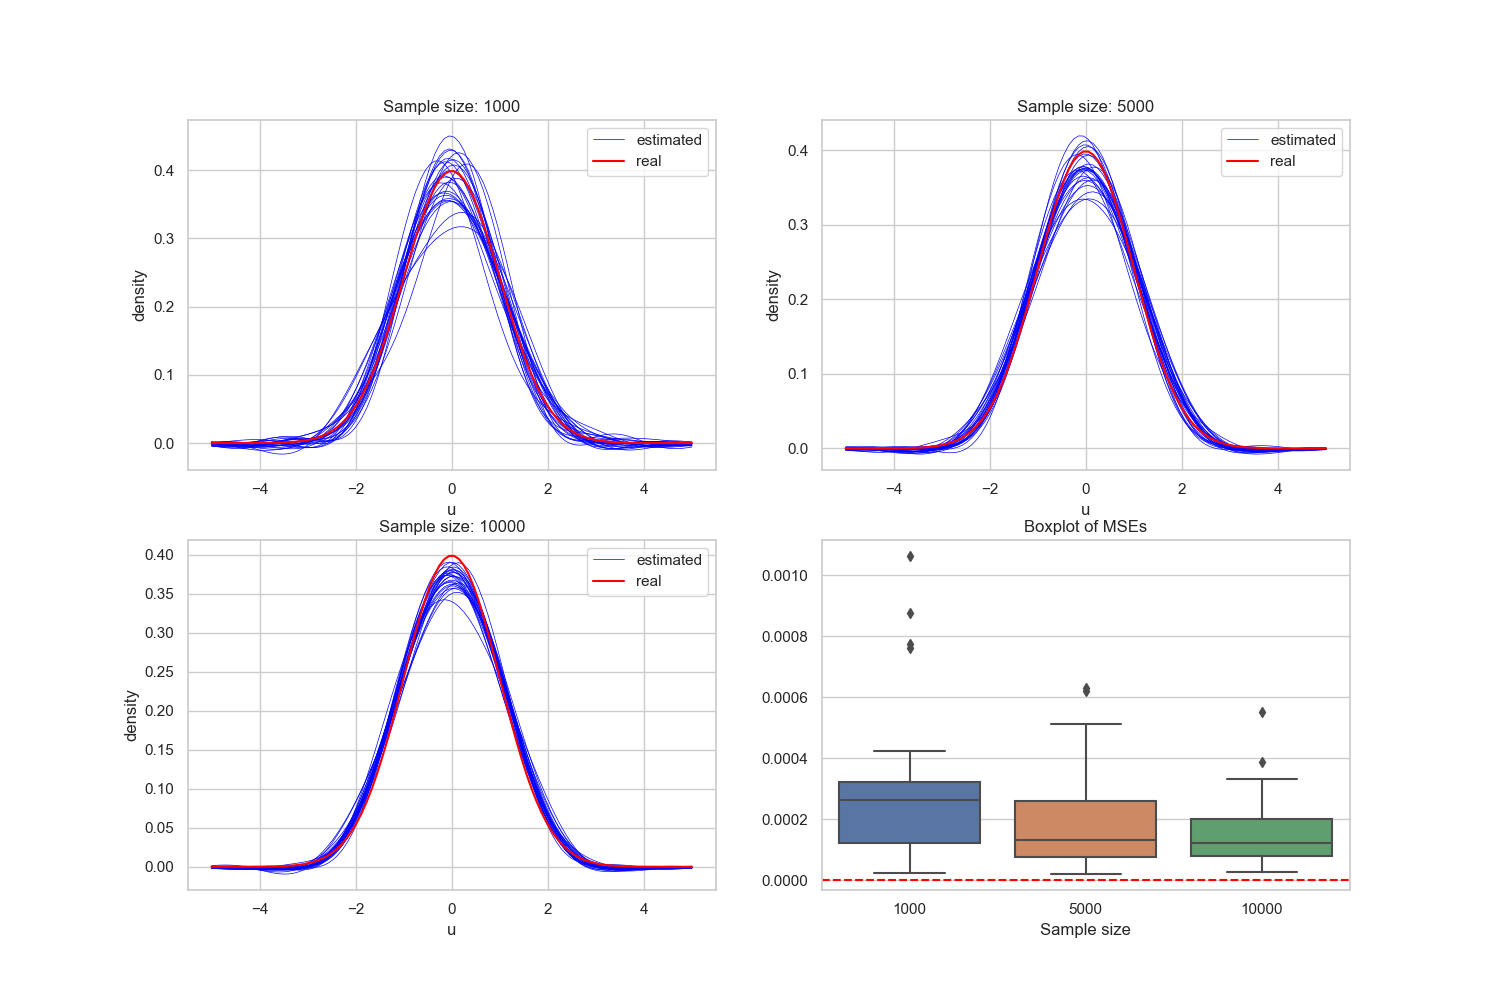
\includegraphics[width=\textwidth]{/Users/mmenadzhiev/Desktop/Studying/Project/Estimation of the media attention/Data/densities.png}
    \caption{Estimated density $p$}
\end{figure}

It is important to note that Figure 7 shows only real part of estimated points but ignoring imaginary part is not fatal because it is approximately zero. Also it is evident that this tendency is strengthening with a growth of a sample size.

\begin{figure}[H]
    \centering
    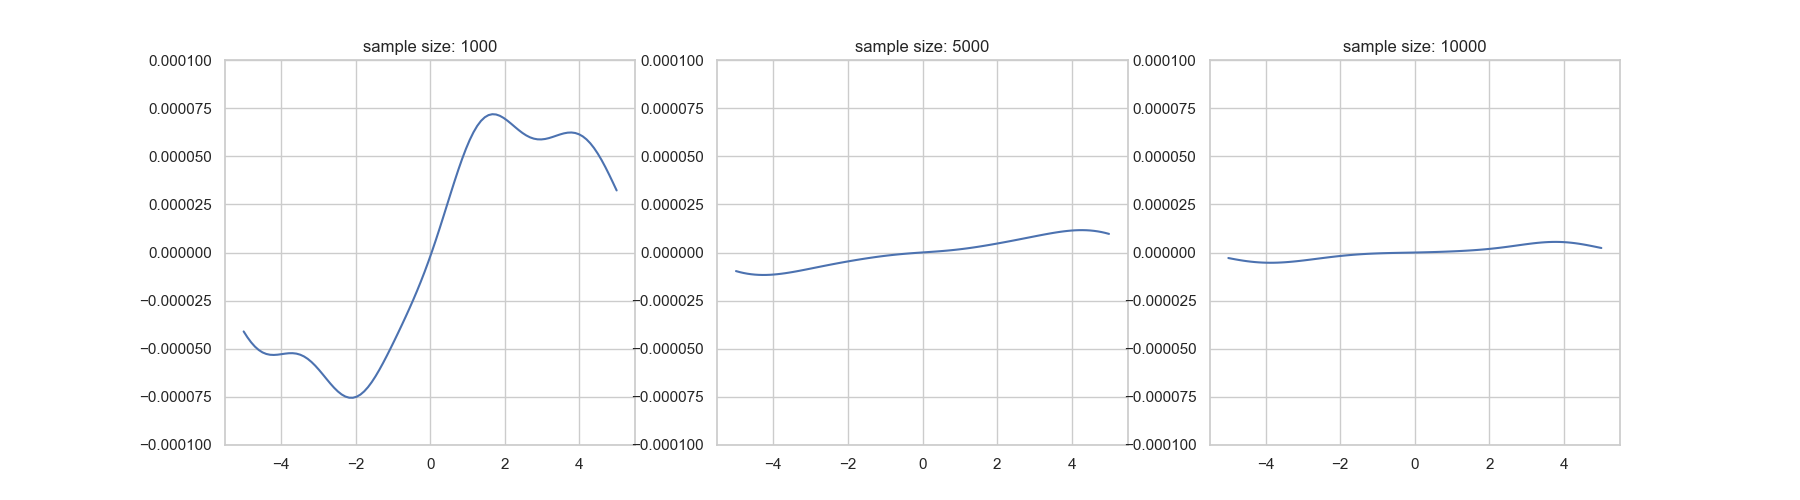
\includegraphics[width=\textwidth]{/Users/mmenadzhiev/Desktop/Studying/Project/Estimation of the media attention/Data/imaginary_part.png}
    \caption{Imaginary parts of $\hat{p}_n (x_s)$}
\end{figure}

\subsection{REAL DATA}

An estimation based on real data requires only a sample which I have obtained from Google Trends. 

\begin{figure}[H]
    \centering
    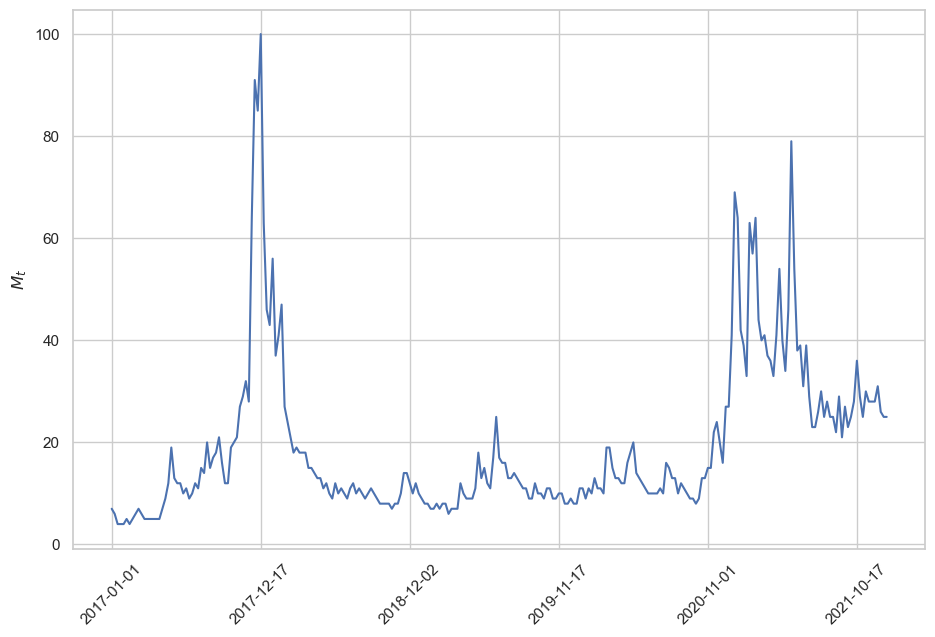
\includegraphics[width=\textwidth]{/Users/mmenadzhiev/Desktop/Studying/Project/Estimation of the media attention/Data/real_M_kDel.png}
    \caption{Media attention index $M_t$ based on real data}
\end{figure}

\begin{figure}[H]
    \centering
    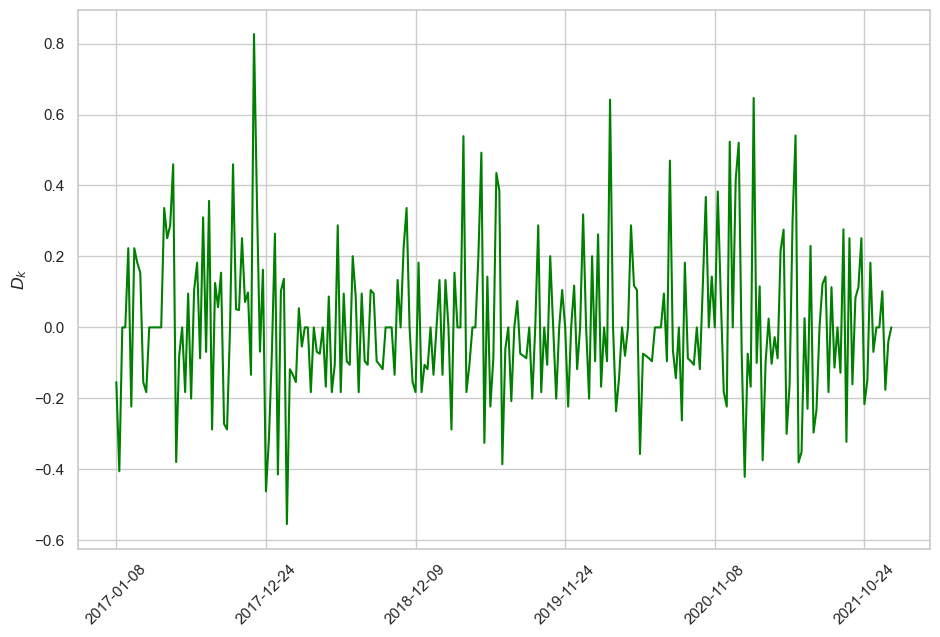
\includegraphics[width=\textwidth]{/Users/mmenadzhiev/Desktop/Studying/Project/Estimation of the media attention/Data/real_D_k.png}
    \caption{Increments $D_k$ based on real data}
\end{figure}

\section{SOME SECTION}

\subsection{CHARACTERISTIC FUNCTION OF NORMAL DISTRIBUTION}

Let $\xi \sim \mathcal N (0, 1)$. Then characteristic function of $\xi$ is \[ f(u) := \E{e^{iu\xi}} = \intR e^{iux} p_{\xi}(x) dx = \frac{1}{\sqrt{2 \pi}} \int_{\R} e^{iux - \frac{x^2}{2}} dx. \] Therefore \[ f'(u) = \frac{i}{\sqrt{2 \pi}} \intR x e^{iux - \frac{x^2}{2}} dx = - \frac{i}{\sqrt{2 \pi}} \intR e^{iux} d e^{-\frac{x^2}{2}} = - \frac{i}{\sqrt{2 \pi}} \left( e^{iux - \frac{x^2}{2}} \big|_{-\infty}^{+\infty} - \intR e^{-\frac{x^2}{2}} d e^{iux} \right) = \] \[ = \Bigg| \Bigg| \left| e^{iux - \frac{x^2}{2}} \right| = e^{-\frac{x^2}{2}} \longrightarrow 0 \text{ as } x \rightarrow \pm \infty \Bigg| \Bigg| = \] \[ = - \frac{u}{\sqrt{2 \pi}} \intR e^{iux - \frac{x^2}{2}} dx = -u f(u). \] Thus, $f(u) = e^{-\frac{u^2}{2}} + c, \text{ } c \in \R.$ Using $f(0) = 1$ we get $c = 0$ and then $f(u) = e^{-\frac{u^2}{2}}$, $u \in \R$.

In case of $\xi \sim \mathcal N (\mu, \sigma^2)$ the characteristic function of $\xi$ is \[ f(u) = \E{e^{iu\xi}} = \frac{1}{\sqrt{2 \pi}} \intR e^{iux} e^{-\frac{(x - \mu)^2}{2 \sigma^2}} dx. \] Also \[ f'(u) = \frac{i}{\sqrt{2 \pi}} \intR x e^{iux} e^{-\frac{(x - \mu)^2}{2 \sigma^2}} dx = \frac{i}{\sqrt{2 \pi}} \intR (x - \mu + \mu) e^{iux} e^{-\frac{(x - \mu)^2}{2 \sigma^2}} dx = \] \[ = \frac{i}{\sqrt{2 \pi}} \left[ \intR (x - \mu) e^{iux} e^{-\frac{(x - \mu)^2}{2 \sigma^2}} dx + \mu \intR e^{iux} e^{-\frac{(x - \mu)^2}{2 \sigma^2}} dx \right] = \frac{i}{\sqrt{2 \pi}} \left[ - \sigma^2 \intR e^{iux} d e^{-\frac{(x - \mu)^2}{2 \sigma^2}} + \mu \sqrt{2 \pi} f(u) \right] \] \[ = \Bigg| \Bigg| \intR e^{iux} d e^{-\frac{(x - \mu)^2}{2 \sigma^2}} = e^{iux - \frac{(x - \mu)^2}{2 \sigma^2}} \Big|_{-\infty}^{+\infty} - i u \intR e^{iux - \frac{(x - \mu)^2}{2 \sigma^2}} dx = - iu \sqrt{2 \pi} f(u) \Bigg| \Bigg| = \] \[ = \frac{i}{\sqrt{2 \pi}} \left[ i \sigma^2 u \sqrt{2 \pi} f(u) + \mu \sqrt{2 \pi} f(u) \right] = \left( i \mu - \sigma^2 u \right) f(u). \]

Therefore \[ f(u) = e^{\int \left( i \mu - \sigma^2 u \right) du } = e^{i \mu u - \frac 12 \sigma^2 u^2 + c}, \text{ } c \in \R. \]

Similarly to the previous case $f(0) = 1$. Thus, $c = 0$ and $f(u) = e^{i \mu u - \frac 12 \sigma^2 u^2}$, $u \in \R$.

\end{document}